\documentclass[12pt,]{book}
\usepackage[]{tgpagella}
\usepackage{amssymb,amsmath}
\usepackage{ifxetex,ifluatex}
\usepackage{fixltx2e} % provides \textsubscript
\ifnum 0\ifxetex 1\fi\ifluatex 1\fi=0 % if pdftex
  \usepackage[T1]{fontenc}
  \usepackage[utf8]{inputenc}
\else % if luatex or xelatex
  \ifxetex
    \usepackage{mathspec}
  \else
    \usepackage{fontspec}
  \fi
  \defaultfontfeatures{Ligatures=TeX,Scale=MatchLowercase}
\fi
% use upquote if available, for straight quotes in verbatim environments
\IfFileExists{upquote.sty}{\usepackage{upquote}}{}
% use microtype if available
\IfFileExists{microtype.sty}{%
\usepackage{microtype}
\UseMicrotypeSet[protrusion]{basicmath} % disable protrusion for tt fonts
}{}
\usepackage[margin=1in]{geometry}
\usepackage{hyperref}
\hypersetup{unicode=true,
            pdftitle={The Realignment of Rebel Groups},
            pdfauthor={David Bowden},
            pdfborder={0 0 0},
            breaklinks=true}
\urlstyle{same}  % don't use monospace font for urls
\usepackage{longtable,booktabs}
\usepackage{graphicx,grffile}
\makeatletter
\def\maxwidth{\ifdim\Gin@nat@width>\linewidth\linewidth\else\Gin@nat@width\fi}
\def\maxheight{\ifdim\Gin@nat@height>\textheight\textheight\else\Gin@nat@height\fi}
\makeatother
% Scale images if necessary, so that they will not overflow the page
% margins by default, and it is still possible to overwrite the defaults
% using explicit options in \includegraphics[width, height, ...]{}
\setkeys{Gin}{width=\maxwidth,height=\maxheight,keepaspectratio}
\IfFileExists{parskip.sty}{%
\usepackage{parskip}
}{% else
\setlength{\parindent}{0pt}
\setlength{\parskip}{6pt plus 2pt minus 1pt}
}
\setlength{\emergencystretch}{3em}  % prevent overfull lines
\providecommand{\tightlist}{%
  \setlength{\itemsep}{0pt}\setlength{\parskip}{0pt}}
\setcounter{secnumdepth}{5}
% Redefines (sub)paragraphs to behave more like sections
\ifx\paragraph\undefined\else
\let\oldparagraph\paragraph
\renewcommand{\paragraph}[1]{\oldparagraph{#1}\mbox{}}
\fi
\ifx\subparagraph\undefined\else
\let\oldsubparagraph\subparagraph
\renewcommand{\subparagraph}[1]{\oldsubparagraph{#1}\mbox{}}
\fi

%%% Use protect on footnotes to avoid problems with footnotes in titles
\let\rmarkdownfootnote\footnote%
\def\footnote{\protect\rmarkdownfootnote}

%%% Change title format to be more compact
\usepackage{titling}

% Create subtitle command for use in maketitle
\newcommand{\subtitle}[1]{
  \posttitle{
    \begin{center}\large#1\end{center}
    }
}

\setlength{\droptitle}{-2em}
  \title{The Realignment of Rebel Groups}
  \pretitle{\vspace{\droptitle}\centering\huge}
  \posttitle{\par}
  \author{David Bowden}
  \preauthor{\centering\large\emph}
  \postauthor{\par}
  \predate{\centering\large\emph}
  \postdate{\par}
  \date{June 30, 2017}

\usepackage{setspace}

\usepackage{float}
\let\origtable\table
\let\endorigtable\endtable
\renewenvironment{table}[1][2] {
    \singlespacing
    \expandafter\origtable\expandafter[H]
} {
    \endorigtable
}

\frontmatter

\usepackage{amsthm}
\newtheorem{theorem}{Theorem}[chapter]
\newtheorem{lemma}{Lemma}[chapter]
\theoremstyle{definition}
\newtheorem{definition}{Definition}[chapter]
\newtheorem{corollary}{Corollary}[chapter]
\newtheorem{proposition}{Proposition}[chapter]
\theoremstyle{definition}
\newtheorem{example}{Example}[chapter]
\theoremstyle{remark}
\newtheorem*{remark}{Remark}
\begin{document}
\maketitle

\doublespacing

\mainmatter

Having explored the formation of new rebel groups in the previous
chapter, I turn now to the other major process affecting the number of
rebel groups in a conflict --- the realignment of existing rebel
factions. There are two ways in which rebels can realign. First, subsets
of existing groups can break away to form splinter organizations. For
example, Hezbollah split from the Amal movement during the Lebanese
Civil War to form a more radical organization. I define a splinter
organization as an independent rebel group, signified by having an
identifiable name and leadership that are not shared with any other
rebel group, that was previously subsumed within another rebel
organization. Thus, entirely new rebel groups are excluded, even if they
constitute a subset of a larger non-violent organization. Splinter
organizations generally emerge during ongoing conflicts, though
sometimes they are formed during periods of peace to initiate a new wave
of fighting, as the Real Irish Republican Army did (Stedman
\protect\hyperlink{ref-Stedman1997}{1997}).

Second, previously independent rebel organizations can form alliances.
Here I focus on alliances with meaningful integration of command
structures, defining an alliance as an organization with a distinct name
that merges a substantial amount of the decision-making for two or more
previously independent rebel groups. This might occur if one group
absorbs another, or two groups create a formal umbrella organization to
coordinate their activities. An example of the latter case is the Syrian
Defense Forces, under which the Kurdish People's Protection Units (YPG)
have joined with several Arab rebel groups to coordinate their campaign
against the Islamic State. Note that this definition excludes
cooperation that falls short of formal integration. Such behavior is
difficult to measure systematically, though multiple forthcoming data
collections should facilitate research on the topic in the future.

I expect these process to be closely related as part of a broader
process of realignment around ethnic identity. Repression should make
civilians more likely to identify with their ethnic group. While I do
not necessarily expect this effect to extend directly to rebels ---
almost by definition, they experience violence --- I do expect that
there will generally be a strong connection between rebels and civilians
dissidents. Except for a few cases with exceptionally large endowments
of natural resources or foreign support, rebels depend on dissident
civilians for recruits, shelter, and material resources. As civilians
often have the ability to defect to the side of a rival rebel group or
the government, rebels have an incentive to represent the interests and
identities of these constituents. Furthermore, ethnic identification can
be an effective means of securing support from foreign co-ethnic states,
and such appeals might be especially likely to succeed during periods of
repression. Thus, rebels should tend to identify more strongly with
their ethnic group following episodes of repression.

This dynamic should lead rebels to reorganize on the basis of ethnicity.
In some cases rebel leaders may be able to reorient their group to
emphasize ethnicity more strongly (see Christia
\protect\hyperlink{ref-Christia2012}{2012}). Often, however, it will be
difficult for them to do so credibly. For example, if a rebel had
previously maintained a multi-ethnic coalition of support, it would be
difficult for them to emphasize a particular ethnic identity. In such
cases, entrepreneurial members of the group may see opportunities to
form a new splinter organization that ``outbids'' the original rebel
group with a more credible, extreme appeal to ethnic identity (see
Horowitz \protect\hyperlink{ref-horowitz85}{1985}). As doing so could
potentially win the support of a large number of dissident civilians,
and leading a rebel group is likely to bring private benefits such as
resource revenues, this should often be an enticing opportunity. As I
expect this cycle of ethnic outbidding to be especially likely in the
wake of repression, I expect that the level of repression should predict
the likelihood that new splinter organizations will form.

\emph{Hypothesis 6: The probability that rebels groups splinter should
increase with the level of repression in a country}

I argue that splintering often reflects a process of reorganization
around ethnic identity. The ability of this process to produce new rebel
groups should depend, however, on the pre-existing configuration. A
rebel group that is already composed primarily of members of a single
ethnicity may be able to adapt to increased ethnic identification,
though they may still fragment as a result of outbidding appeals.
Nevertheless, groups that draw their support from multiple ethnic groups
should be much more vulnerable to fragmentation as the result of
increased ethnic identification.

\emph{Hypothesis 7: Multi-ethnic rebel groups should be at greater risk
of splintering than mono-ethnic ones}

My theory also suggests a testable implication regarding the
characteristics of the splinters groups that emerge. If splintering is
motivated by a desire to form rebel groups that more clearly represent a
particular ethnic group, the rebel groups that emerge from this process
should be likelier than others to draw their support from a single
ethnic group.

\emph{Hypothesis 8: Splinter organizations should be more likely than
others to draw their support from a single ethnic group}

While this process of realignment around ethnic identities should lead
to the fragmentation of some groups, in other cases it might create
opportunities for aggregation. One disadvantage of splintering is that
it will generally result in a weaker organization than members had
previously, as it will have only a subset of the parent group's members
at its disposal. As a crucial function of alliances is the aggregation
of capabilities, forming new alliances is a potential solution to this
problem. Alliances may also have the benefit of managing potential
conflict between their members (Gibler
\protect\hyperlink{ref-Gibler1996}{1996}), ensuring that resources are
directed toward fighting the government rather than other rebel groups.
Finally, outside states often attempt to maximize the impact of their
support by channeling it to a coalition of rebels, rather than a series
of smaller, independent groups. Interventions of this sort might be
especially likely in the wake of a humanitarian crisis.

As is the case with splintering, my theory offers predictions regarding
not only when new alliances should emerge, but also what their ethnic
composition should be. I expect that the ethnic polarization sparked by
repression should lead rebels to leave multi-ethnic coalitions, but also
to form new alliances with co-ethnic factions.

\emph{Hypothesis 9: The probability that new, mono-ethnic alliances will
form should increase with the level of repression}

Conversely, the emergence of multi-ethnic alliances should be less
likely when this dynamic is at work.

\emph{Hypothesis 10: The probability that new, multi-ethnic alliances
will form should decrease with the level of repression}

\section{Research Design}\label{research-design}

While I believe them to be the result of closely related theoretical
processes, the splintering of individual rebel organizations and the
formation of alliances between separate organizations require distinct
research designs. I first explain my choice of designs for studying
splintering.

\subsection{Splintering}\label{splintering}

The first phenomenon I explain in this chapter is splintering. As the
explanatory factors in \emph{H7} and \emph{H8} are group attributes, the
unit of analysis in this portion of the study is the rebel group-year. I
seek to explain not simply which conflict years produce splinter
organizations, but also which rebel groups within those conflict years.
I draw my sample of cases from the UCDP Dyadic Dataset, version 4-2016
(Melander, Pettersson, and Themnér
\protect\hyperlink{ref-Melander2016}{2016}), which includes an
observation for every non-state actor in every year in which it was
involved in conflict with the government producing at least 25
fatalities. After collapsing observations for rebel groups that appear
in multiple conflicts in a single year, I am left with a dataset of
2,656 rebel group years covering the period 1946--2015.

\subsubsection*{Dependent Variables}\label{dependent-variables}
\addcontentsline{toc}{subsubsection}{Dependent Variables}

\textbf{Splintering}

The first dependent variable in this portion of the analysis is the
splintering of existing rebel groups. I use my own data on rebel group
origins to identify splinter groups.\footnote{The UCDP Actor data
  (Uppsala Conflict Data Program
  \protect\hyperlink{ref-ucdpactor}{2015}) does identify splinter
  groups, but uses very conservative coding rules that exclude many
  clear examples of splinter.} A group is coded as a splinter
organization if most of its leadership were previously members of
another rebel group. I follow the UCDP coding decisions for
distinguishing cases where a new group has emerged from simple name
changes. Essentially, a group is considered new if its leadership,
organizational structure, or membership differs substantially from
previous existing organizations. When two groups disagree about which is
the original organization and which is the splinter, the larger group is
considered the original.

113 of the 506 rebel groups in my data are splinter organizations. As
there are four cases in which a rebel group produced two splinter
organizations in the same year, the number of years in which a new
splinter organization emerged is 109. However, a large portion of these
are coterminous with dissolution of the original organization. Typically
in these cases the main organization will agree to a peace deal, and a
radical faction will form a splinter organization to continue fighting.
While this is an interesting and consequential phenomenon, it has
already received a substantial amount of attention from scholars (e.g.
Stedman \protect\hyperlink{ref-Stedman1997}{1997}). Furthermore, I am
interested in processes that increase or decrease the number of rebel
groups in a conflict. Replacing a large, moderate organization with a
more radical splinter has important implications for the probability of
peace and the tactics likely to be deployed. Ultimately, however, it
does not alter the number of rebel groups competing simultaneously. I
thus consider these cases to be beyond the scope of this dissertation,
and exclude them from my analyses. This leaves a total of 25 cases in
which a splinter and parent organization were active simultaneously.
This variable is coded as 1 in the group-year in which a parent
organization loses a splinter faction (i.e.~I examine the groups that
splinter).

\textbf{Rebel Group Ethnicity}

\emph{H8} predicts that splinter organizations should be more likely
than others to draw support from a single ethnic group. As I did for the
similar hypothesis in Chapter \ref{entry}, I use the the ACD2EPR 2014
dataset (Wucherpfennig et al.
\protect\hyperlink{ref-Wucherpfennig2011}{2011}; Vogt et al.
\protect\hyperlink{ref-Vogt2015}{2015}) to determine this. The data
measures three categories of ties between rebel and ethnic groups ---
explicit claims of representation, recruiting, and support from at least
half the ethnic group. I collapse these forms to code a trichotomous
measure indicating whether a rebel group is multi-ethnic, mono-ethnic,
or non-ethnic, meaning it has no observable links to any ethnic group.

\subsubsection*{Independent Variables}\label{independent-variables}
\addcontentsline{toc}{subsubsection}{Independent Variables}

\textbf{Human Rights}

I again use the Latent Human Protection scores, version 2 (Fariss
\protect\hyperlink{ref-Fariss2014}{2014}; Schnakenberg and Fariss
\protect\hyperlink{ref-Schnakenberg2014}{2014}) to measure repression.
As I do in Chapter \ref{entry}, I combat the fact that the measure is
mostly static with a slight positive trend over time by using the change
over the previous. In this measure, a negative score indicates that a
country has become more repressive, while a positive score means that
human rights have improved. In this sample the mean change is just 0.01,
but there are numerous large change in both directions.

\textbf{Multi-ethnic Group}

To test \emph{H7} I use the measure of rebel group ethnicity that serves
as a dependent variable later in the chapter. In this case I collapse
the measure into a dichotomous indicator with rebel groups that draw
support from multiple ethnic groups coded as 1, and all others coded as
zero. There are relatively few multi-ethnic groups in the data, with the
attribute occurring in 334 of 2393 valid group-year observations.

\textbf{Splinter Organization}

The test of \emph{H8} uses the splinter variable from my rebel origins
data as an explanatory factor. The coding rules are described above. 113
out of 503 rebel groups are splinter organizations.

\subsubsection*{Control Variables}\label{control-variables}
\addcontentsline{toc}{subsubsection}{Control Variables}

I include many of the country-level covariates from Chapter \ref{entry}
in the splintering analyses as controls. These include ethnolinguistic
fractionalization (Fearon and Laitin
\protect\hyperlink{ref-fearonlaitin03}{2003}), Polity IV score
(Marshall, Gurr, and Jaggers
\protect\hyperlink{ref-Marshall2016}{2016}), land area (The World Bank
\protect\hyperlink{ref-WorldBank2015}{2015}), population (Gleditsch
\protect\hyperlink{ref-Gleditsch2002b}{2002}), GDP per capita (Gleditsch
\protect\hyperlink{ref-Gleditsch2002b}{2002}), and a count of lootable
resource sites (Lujala, Rød, and Thieme
\protect\hyperlink{ref-Lujala2007}{2007}; Gilmore et al.
\protect\hyperlink{ref-Gilmore2007}{2005}; Lujala, Gleditsch, and
Gilmore \protect\hyperlink{ref-Lujala2005}{2005}; Balestri
\protect\hyperlink{ref-Balestri2012}{2012}; Lujala
\protect\hyperlink{ref-Lujala2008}{2008}; Buhaug and Lujala
\protect\hyperlink{ref-Buhaug2005}{2005}). Refer to the previous chapter
for detailed descriptions.

Additionally I include several rebel group-level controls from
Cunningham, Gleditsch, and Salehyan
(\protect\hyperlink{ref-Cunningham2009}{2009}). These include a binary
indicators of whether the rebel group is stronger than the government,
whether the group has a presence in multiple states, whether the group
has a political wing, whether the group controls territory, whether the
group has centralized control, and whether it receives external support.
Each of these measures is a snapshot, measured for each group at only
one point in time.

\subsubsection*{Modeling Strategies}\label{modeling-strategies}
\addcontentsline{toc}{subsubsection}{Modeling Strategies}

To test \emph{H6} and \emph{H7} I use a Cox proportional hazard survival
model. This is a useful modeling framework in this case because the
probability that a rebel group will splinter is in part a function of
time. In a standard logistic regression analysis with the rebel group as
the unit of analysis, the duration of time the group was active is such
a strong predictor of splintering that it typically nullifies the
significance of all other variables. Survival models address this by
treating splintering as a function of time, expressed as the probability
that a rebel group will survive a given number of years without
splintering. Independent variables explain deviations from this baseline
survival curve. The Cox model is likely to be the proper choice of
survival models in this case, as survival times for rebel groups are
heavily right-skewed, and the Cox model does not assume survival times
form any particular distribution (i.e.~it is non-parametric).

The exact specification of the dependent variable in this analysis is
the number of years between a rebel group's first appearance in the data
and the first time it generates a splinter organization. I remove a
rebel group from the study once it has splintered for the first time.
This results in the exclusion of three instances of splintering from
rebel groups that had splintered previously. As many of my covariates
are measured at the country level and there are often multiple rebel
groups per country, I cluster the standard errors by country.

To test \emph{H8} I use a simple logistic regression with the rebel
group as the unit of analysis. The mono-ethnic indicator is the
dependent variable, and the indicator of whether the group is a splinter
organization is the main predictor.

\subsection{Alliance Formation}\label{alliance-formation}

The research design for the two alliance formation hypotheses (\emph{H9}
and \emph{H10}) closely resembles the group formation analysis from
Chapter \ref{entry}. The unit of analysis is the conflict-year. While I
control for the number of rebel groups, I do not exclude observations
that have only one rebel group. There are several cases where a new
rebel group enters a conflict and joins an alliance in the same calendar
year.

\subsubsection*{Dependent Variable}\label{dependent-variable}
\addcontentsline{toc}{subsubsection}{Dependent Variable}

The dependent variables for the two hypotheses are the formation of two
different types of alliances --- mono-ethnic and multi-ethnic. I use my
data on rebel origins to determine when a new alliance has formed. I
code an alliance as any group whose members are drawn from at least two
distinct previously active rebel groups. These alliances constitute a
substantial enough integration of command that they replace their
constituent groups in the data. In many cases, however, the alliance
splinters and the members groups re-enter the data. I combine the
alliance measure with the ethnic composition variable to code two
dependent variables --- the formation of new multi-ethnic alliances, and
of new mono-ethnic ones. Alliances involving this degree of integration
are rare. New mono-ethnic alliances form in 29 of 2014 conflict-years,
while there are only 13 years in which a new multi-ethnic alliance
emerged.

\subsubsection*{Independent Variable}\label{independent-variable}
\addcontentsline{toc}{subsubsection}{Independent Variable}

I use same measure of human rights as in the preceding analyses. I again
use the lagged change in the Latent Human Protection Score (Fariss
\protect\hyperlink{ref-Fariss2014}{2014}; Schnakenberg and Fariss
\protect\hyperlink{ref-Schnakenberg2014}{2014}). The mean change in this
data is -0.01, with a range from -2.51 to 1.50.

\subsubsection*{Control Variables}\label{control-variables-1}
\addcontentsline{toc}{subsubsection}{Control Variables}

I include two conflict-level controls: a binary indicator of whether the
conflict produced 1,000 or more fatalities in a year, and a binary
indicator of whether multiple rebel groups participated in the conflict
in a year. Both measures come from the UCDP Dyadic Data (Melander,
Pettersson, and Themnér \protect\hyperlink{ref-Melander2016}{2016}).
Additionally I control for several country-level factors, including
ethnolinguistic fractionalization and the percentage of terrain that is
mountainous (Fearon and Laitin
\protect\hyperlink{ref-fearonlaitin03}{2003}), population and GDP per
capita (Gleditsch \protect\hyperlink{ref-Gleditsch2002b}{2002}), the
Polity IV score (Marshall, Gurr, and Jaggers
\protect\hyperlink{ref-Marshall2016}{2016}), and an indicator of whether
there was a civil war in a neighboring country.

\subsubsection*{Modeling Strategy}\label{modeling-strategy}
\addcontentsline{toc}{subsubsection}{Modeling Strategy}

As both dependent variables are binary but rare, I use a logistic
regression with a rare events correction (King and Zeng
\protect\hyperlink{ref-King2001a}{2001}). As there are sometimes
multiple conflicts in a country-year, I cluster the standard errors by
country.

\section{Splintering Results}\label{splintering-results}

Results of the splintering analysis are reported in Table
\ref{tab:survival}. I fit five Cox proportional hazard models with
different batteries of covariates. Model 1 includes only the two
independent variables used to test my hypotheses --- the lagged change
in human rights, and an indicator of whether the rebel group is
multi-ethnic. In Model 2 I add several country-level control variables.
Model 3 combines the change in human rights with a set of rebel
group-level controls.

\begin{table}
\begin{center}
\begin{tabular}{l c c c }
\hline
 & Model 1 & Model 2 & Model 3 \\
\hline
Change in Human Rights            & $-1.23^{\dagger}$ & $-1.34$  & $-1.35^{\dagger}$ \\
                                  & $(0.74)$          & $(0.94)$ & $(0.81)$          \\
Multi-ethnic Group                & $0.54$            & $-0.14$  & $0.55$            \\
                                  & $(0.65)$          & $(1.01)$ & $(0.54)$          \\
Polity                            &                   & $-0.02$  &                   \\
                                  &                   & $(0.05)$ &                   \\
Logged GDPpc                      &                   & $0.17$   &                   \\
                                  &                   & $(0.36)$ &                   \\
Logged Population                 &                   & $-0.44$  &                   \\
                                  &                   & $(0.30)$ &                   \\
Logged Area                       &                   & $0.08$   &                   \\
                                  &                   & $(0.40)$ &                   \\
Ethnolinguistic Fractionalization &                   & $0.85$   &                   \\
                                  &                   & $(1.16)$ &                   \\
Lootable Resource Sites           &                   & $0.01$   &                   \\
                                  &                   & $(0.01)$ &                   \\
Intensity Level                   &                   & $-1.34$  &                   \\
                                  &                   & $(1.06)$ &                   \\
Transnational Group               &                   &          & $0.39$            \\
                                  &                   &          & $(0.87)$          \\
Political Wing                    &                   &          & $-0.56$           \\
                                  &                   &          & $(0.46)$          \\
Stronger than Gov.                &                   &          & $2.05^{*}$        \\
                                  &                   &          & $(0.92)$          \\
\hline
AIC                               & 171.59            & 101.72   & 145.35            \\
R$^2$                             & 0.00              & 0.00     & 0.00              \\
Max. R$^2$                        & 0.09              & 0.06     & 0.08              \\
Num. events                       & 20                & 12       & 17                \\
Num. obs.                         & 1908              & 1499     & 1740              \\
Missings                          & 749               & 1158     & 917               \\
PH test                           & 0.06              & 0.59     & 0.74              \\
\hline
\multicolumn{4}{l}{\scriptsize{$^{***}p<0.001$, $^{**}p<0.01$, $^*p<0.05$, $^{\dagger}p<0.1$}}
\end{tabular}
\caption{Cox Proportional Hazard Models of Rebel Group Splintering}
\label{tab:survival}
\end{center}
\end{table}

The coefficients of a Cox model represent the effect of a variable on
the hazard of failure (splintering in this case). A positive coefficient
indicates that the risk of splintering increases with the level of that
variable, while a negative coefficients signifies a reduced risk.
Consistent with \emph{H6} I find that the change in human rights is
negatively related to the hazard of splintering. As human rights improve
the risk that a rebel group will splinter decreases; as a country
becomes more repressive, the risk of splintering increases. However, the
effect is only statistically significant in Models 1 and 4, and even
then only at the 90\% level. The effect size is large, with a one-unit
increase in human rights being associated with a 70\% reduction in the
likelihood of splintering in Model 1, and a 74\% reduction in Model 4.
The relationship is not significant in Model 2, though it is not clear
whether the relationship is confounded by the country-level covariates,
or the change is the result of missing data on those variables.

The findings are thus mostly consistent with \emph{H6}, though not as
robust as most of the analyses in the preceding chapters. Several cases
from the data clearly fit my theoretical framework. The Karenni ethnic
group of Burma are close relatives of the Karen, and fought as members
of the Karen National Union (KNU) for the first several years of Burmese
independence. In 1957, however, the Karenni left the KNU to form their
own rebel group, the Karenni National Progressive Party (KNPP). This
case illustrates that splintering does not always lead to hostile
relations between the formerly united groups, however, as the KNU
strongly supported the KNPP's desire to pursue a separate Karenni state
(Fredholm \protect\hyperlink{ref-Fredholm1993}{1993}). The Free Aceh
Movement splintered from Darul Islam in Indonesia to pursue independence
for the Acehnese people, rather than the Darul Islam's goals of an
Islamic State in Indonesia. A review of the cases also suggests a
possible explanation for the lack of robustness --- communist rebel
groups are highly prone to fragmentation, and account for a large
portion of the splinter organizations.

I find no support for \emph{H7}, as the multi-ethnic variable never
approaches statistical significance. As I discuss in the study of the
Shan State independence movement later in this chapter, it is seemingly
common for ethnically homogeneous groups to splinter. Only one control
variable is significant --- the indicator of whether a rebel group is
stronger than the government in Model 3. Being stronger than the
government increases the risk of splintering by a factor of seven. This
suggests that splintering has a strong strategic element. When rebels
are weak and cannot afford any loss in capability, they hang together.
When victory appears likely, however, they act on their internal
differences, perhaps with an eye toward post-war bargaining.

In summary the results of this analysis are largely consistent with my
broader theory, though not robust to the inclusion of country-level
controls. I interpret the results as suggesting that ethnic polarization
is a common pathway to splintering. It is not, however, the only
pathway. Communist rebellions are prone to splintering along doctrinal
lines, and splinter organizations often emerge late in conflicts to
continue the fighting after the original organization ceases its
activities.

\subsection{Splinter Group Ethnicity}\label{splinter-group-ethnicity}

\emph{H8} predicts that splinter organizations should be more likely
than others to draw their support from a single ethnic group. If
splintering is fundamentally about reorganization along ethnic lines, it
stands to reason that the leaders of splinter organizations should take
only co-ethnics with them. I test this proposition in Table
\ref{tab:splintcomp}. I do not find support for \emph{H8}, as splinter
organizations are not likely than others (alliances and originating
rebel groups constitute the baseline) to be ethnically-homogeneous.
Splinter organizations also do not significantly differ in their
probability of being multi-ethnic. I do find that splinter organizations
are less likely less likely than others to have no ties to any ethnic
group, with the effect being significant at the 95\% level. This
suggests that support from ethnic constituents might be an important
factor in facilitating splintering. Factions that lack such support may
be more likely to remain in the original rebel group, as they have less
assurance of being able to acquire enough resources to be a viable
independent group.

\begin{table}
\begin{center}
\begin{tabular}{l c c c }
\hline
 & M4 Monoethnic & M5 Multiethnic & M6 Nonethnic \\
\hline
(Intercept)                      & $0.20$       & $-3.70^{***}$ & $-0.04$     \\
                                 & $(0.29)$     & $(0.63)$      & $(0.31)$    \\
Splinter                         & $0.39$       & $0.54$        & $-1.14^{*}$ \\
                                 & $(0.41)$     & $(0.54)$      & $(0.57)$    \\
Joiner                           & $0.75^{*}$   & $-1.08$       & $-0.47$     \\
                                 & $(0.34)$     & $(0.66)$      & $(0.37)$    \\
Secessionist                     & $1.07^{***}$ & $-1.18^{*}$   & $-0.76^{*}$ \\
                                 & $(0.31)$     & $(0.50)$      & $(0.36)$    \\
Previously Active                & $-0.08$      & $0.04$        & $0.17$      \\
                                 & $(0.42)$     & $(0.58)$      & $(0.52)$    \\
Ethnlinguistic Fractionalization & $0.16$       & $2.09^{*}$    & $-1.15^{*}$ \\
                                 & $(0.45)$     & $(0.85)$      & $(0.52)$    \\
Transnational                    & $0.06$       & $1.06^{*}$    & $-0.69^{*}$ \\
                                 & $(0.26)$     & $(0.42)$      & $(0.31)$    \\
\hline
AIC                              & 393.19       & 193.69        & 320.15      \\
BIC                              & 419.59       & 220.09        & 346.55      \\
Log Likelihood                   & -189.60      & -89.85        & -153.07     \\
Deviance                         & 379.19       & 179.69        & 306.15      \\
Num. obs.                        & 321          & 321           & 321         \\
\hline
\multicolumn{4}{l}{\scriptsize{$^{***}p<0.001$, $^{**}p<0.01$, $^*p<0.05$}}
\end{tabular}
\caption{Logit Models of Rebel Group Ethnic Composition}
\label{tab:splintcomp}
\end{center}
\end{table}

\section{Alliance Formation Results}\label{alliance-formation-results}

The alliance formation results are reported in Table \ref{tab:alliance}.
Model 1 uses mono-ethnic alliances as the dependent variable, while
Model 2 focuses on multi-ethnic alliances and Model 3 combines all
alliances. In \emph{H9} I predict that the probability of new ethnically
homogeneous alliance will be greater following increases in repression.
Consistent with this prediction, the ``Change in Human Rights'' variable
has a strong negative relationship with the probability of new rebel
group formation. A one-unit decrease in human rights (again, roughly the
difference between France and Russia in recent years) more than triples
the odds of a new rebel group forming. In the years following the
largest declines in human rights practices (-2.5), the probability of a
new mono-ethnic alliance is 0.21 (see Figure \ref{fig:zeligplot}). When
the change is zero or positive, the probability of such an alliance is
around 0.01. This relationship is statistically significant at the 90\%
level. Given that the sample size is not especially small (n=1209), an
\(\alpha\) of 0.1 might be considered overly permissive. However, no
other variable is significant at even the 90\% level, suggesting that
even after applying the rare events correction the model has limited
statistical power. Thus, I contend that it is reasonable to interpret
relationships at this significance level, and reject the null hypothesis
of no relationship between repression and the emergence of mono-ethnic
rebel groups.

\begin{table}
\begin{center}
\begin{tabular}{l c c c }
\hline
 & M1 Mono-ethnic & M2 Multi-ethnic & M3 All \\
\hline
(Intercept)                       & $1.56$            & $-1.25$   & $1.71$            \\
                                  & $(3.82)$          & $(12.46)$ & $(2.84)$          \\
Change in Human Rights            & $-1.20^{\dagger}$ & $-1.15$   & $-0.99^{\dagger}$ \\
                                  & $(0.70)$          & $(1.26)$  & $(0.55)$          \\
Ethnolinguistic Fractionalization & $0.79$            & $11.27$   & $1.12$            \\
                                  & $(1.21)$          & $(10.54)$ & $(0.95)$          \\
Intensity Level                   & $0.09$            & $0.54$    & $0.03$            \\
                                  & $(0.58)$          & $(0.89)$  & $(0.45)$          \\
Prev. Multi-rebel                 & $-0.42$           & $0.35$    & $0.31$            \\
                                  & $(0.78)$          & $(0.88)$  & $(0.47)$          \\
Contiguous Civil War              & $0.01$            & $0.08$    & $-0.06$           \\
                                  & $(0.15)$          & $(0.28)$  & $(0.13)$          \\
Logged GDP per capita             & $-0.39$           & $-0.78$   & $-0.43^{\dagger}$ \\
                                  & $(0.35)$          & $(1.01)$  & $(0.26)$          \\
Logged Population                 & $-0.33$           & $-0.75$   & $-0.29$           \\
                                  & $(0.26)$          & $(0.70)$  & $(0.20)$          \\
Polity                            & $-0.04$           & $0.00$    & $-0.01$           \\
                                  & $(0.05)$          & $(0.11)$  & $(0.04)$          \\
\hline
AIC                               & 163.10            & 71.96     & 241.14            \\
BIC                               & 214.07            & 122.94    & 292.12            \\
Log Likelihood                    & -71.55            & -25.98    & -110.57           \\
Deviance                          & 143.10            & 51.96     & 221.14            \\
Num. obs.                         & 1209              & 1210      & 1210              \\
\hline
\multicolumn{4}{l}{\scriptsize{$^{***}p<0.001$, $^{**}p<0.01$, $^*p<0.05$, $^{\dagger}p<0.1$}}
\end{tabular}
\caption{Rare Events Logit Models of Alliance Formation}
\label{tab:alliance}
\end{center}
\end{table}

In Model 2 I do not find support for \emph{H10}, as the relationship
between ``Change in Human Rights'' and the probability of new
multi-ethnic alliances does not approach statistical significance. While
repression does not seem to deter this type of alliance as I expected,
neither does it make them more likely. Thus while I find that repression
is associated with a general increase in the probability of new
alliances, the relationship seems to be driven by ethnically-homogeneous
coalitions. The effect of repression seems to be specific to this type
of alliance, rather than producing a general increase in the propensity
to form coalitions.

\begin{figure}
\centering
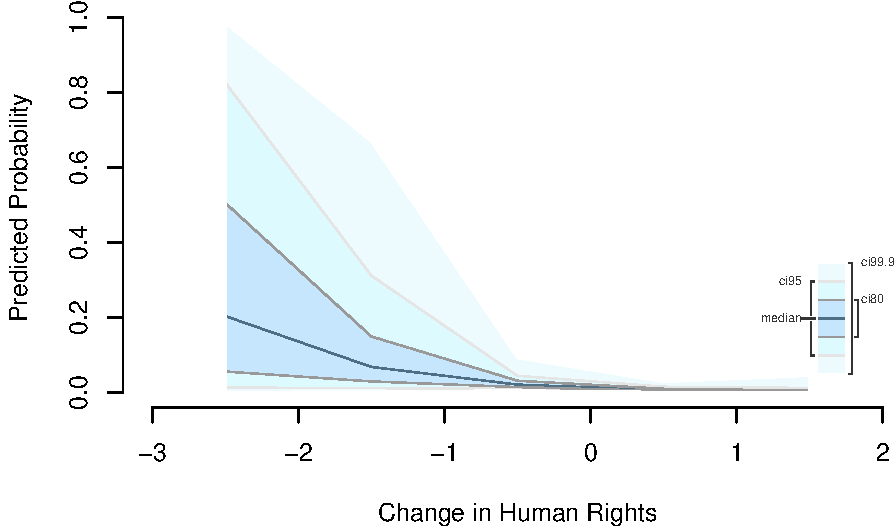
\includegraphics{realignment_standalone_files/figure-latex/zeligplot-1.pdf}
\caption{\label{fig:zeligplot}Predicted Probability of Mono-ethnic Alliance
(Model 1)}
\end{figure}

The only statistically significant control variable in any of the three
models is logged GDP per capita in Model 3. The relationship is
negative, indicating that alliances are less common in wealthier
countries. One possible explanation is that the variable is acting as a
proxy for the intensity or spread of the conflict, capturing an
attribute distinct from the binary measure of whether the conflict
produced 1,000 fatalities. In cases such as Afghanistan where most of
the country is consumed by war, the economy is likely to suffer. In
cases where the fighting is more localized, such as Ukraine in recent
years, there will not necessarily be a significant economic decline at
the country level. The former situation might be more likely to have a
plethora of rebel groups available to form alliances.

The findings in this section are broadly consistent with my theoretical
framework. Increased repression is associated with higher probabilities
of the formation of ethnically homogeneous alliances, which supports my
expectation that repression triggers a cycle of realignment around
ethnic identity. One case that is consistent with this story is the
Uganda National Liberation Front. Uganda is among the most ethnically
diverse societies on earth, with an ethnolinguistic fractionalization
score indicating that there is nearly a 90\% chance that two randomly
selected individuals will be from different ethnic groups. A number of
small rebel groups formed there in 1978 with the goal of overthrowing
Idi Amin, to which the government responded with a substantial increase
in repression (a change of -0.5 in the Latent Human Protection Scores).
In early 1979, with help from the Tanzanian government, several
ethnically Lango rebel groups responded by a forming an alliance, the
Uganda National Liberation Front. A month later they successfully
overthrew Amin. While numerous small rebel groups were active during
this time (Lewis \protect\hyperlink{ref-Lewis2016}{2016}), only the bloc
of Lango groups was able to successfully form an alliance.

\section{The Shan Secessionist
Movement}\label{the-shan-secessionist-movement}

The Shan State secessionist movement in Burma includes cases that
support both the splintering and alliance formation aspects of the
analysis. Yet it has also seen many instances of splintering that my
theory would not predict, suggesting additional variables for
consideration. Shan State is a large, mountainous area in eastern Burma,
bordering Thailand on the south, Laos on the east, and China on the
north. The Shan people and language are both closely related to the
Thai, and in pursuit of its historical rivalry with Burma the Thai
government has frequently supported Shan rebellions to form a sort of
buffer zone between the two countries (Steinberg
\protect\hyperlink{ref-Steinberg2010}{2010}). Adding to the
international character of the region are the facts that it has long
been one of the world's most productive areas for opium cultivation, and
that it was used as refuge by Kuomintang (KMT) forces fleeing China in
the 1950's and 1960's (Cowell \protect\hyperlink{ref-Cowell2005}{2005}).
Shan State initially faced less repression than most other areas of the
country, as it had been granted the right to secede in the Burmese
Constitution (Silverstein
\protect\hyperlink{ref-Silverstein1958}{1958}).

The initial formation of rebellion in Shan State is largely consistent
with the process of group formation I discuss in Chapter \ref{entry},
although there was not an ongoing conflict in the region. Following
their defeat in the Chinese Civil War in 1950, a contingent of KMT
soldiers fled into Shan in search of refuge. During the same period, the
Communist Party of Burma and separatists from the Kachin region
frequently used the area as a base of operations (Smith
\protect\hyperlink{ref-Smith1999}{1999}). In hopes of defeating the
Communists and Kachin, and expelling the KMT, the Burmese army sent a
large troop deployment to the region in the late 1950's. These forces
were undisciplined, however, and frequently committed abuses against the
local population. These abuses induced a greater level of Shan
nationalism as a basis for opposition to the occupation (Fredholm
\protect\hyperlink{ref-Fredholm1993}{1993}, Ch. 8). The process of
increased ethnic identification in this case is largely consistent with
my theoretical argument. Shan elites, especially the leaders of student
organizations, began developing and advocating for a distinctly Shan
identity in the mid-1950's. Repression by the Burmese army significantly
enhanced the efficacy of these appeals, leading large portions of the
Shan to embrace ethnic nationalism (Fredholm
\protect\hyperlink{ref-Fredholm1993}{1993}, 156--57). In 1958 this
nationalism culminated in the formation of the first Shan rebel group,
the Young Brave Warriors.

Shortly after the fighting began, the Young Brave Warriors splintered. A
large portion of the group's membership joined the new Shan State
Independence Army (SSIA). One factor in this move appears to be the fact
that the SSIA was more explicitly nationalist than its predecessor
(Brown \protect\hyperlink{ref-Brown1988a}{1988}; Fredholm
\protect\hyperlink{ref-Fredholm1993}{1993}, 156). While I expect
ethnically-homogeneous groups such as the Young Brave Warriors to be
more cohesive than multi-ethnic coalitions, these groups are still
vulnerable to outbidding appeals. The Young Brave Warriors-SSIA split is
consistent with my general argument that repression induces greater
levels of ethnic identification, which in turn leads rebels to
reorganize. It also suggests an explanation for my finding of no
relationship between the ethnic composition of a rebel group and its
risk of splintering --- even ethnically-homogeneous groups are at risk
of splintering through an outbidding dynamic. Thus it may be the case
that the null finding is the result not of multi-ethnic groups being
cohesive, but rather of mono-ethnic groups being similarly fragile.

The Shan secessionist movement has also seen the creation of several
alliances. Almost immediately upon splitting from the Young Brave
Warriors, the students who from the SSIA welcomed a group of defectors
from the Burmese Army (Fredholm
\protect\hyperlink{ref-Fredholm1993}{1993}, 156). In 1964, the SSIA
participated in a much larger merger with the Kokang Force and the Shan
National United Front, forming the Shan State Army (SSA) (Lintner
\protect\hyperlink{ref-Lintner1984}{1984}). While the Kokang are often
considered a separate ethnic group from the Shan, in my data they are
coded as having no ties to an ethnic group. With the other two members
being Shan, the SSA is coded as an instance of a new mono-ethnic
alliance. Collectively, the various Shan organizations totaled no more
than 8,000 members (Fredholm \protect\hyperlink{ref-Fredholm1993}{1993},
158). Thus aggregating and coordinating capabilities was likely an
important motive for the group leaders. The timing of the merger is also
consistent with my theory. Burma's democratic regime fell to a military
coup in 1962, two years prior to the formation of the SSA. While the
Latent Human Protection Scores do not detect a sharp change perhaps due
to a dearth of data sources in that period, the tactics used by the new
military regime toward the various separatists were generally harsher
than those of the previous regime (Charney
\protect\hyperlink{ref-Charney2009}{2009}).

While the early years of the Shan independence movement provide strong
support for my theory, the amount of subsequent splintering observed
there surpasses what I would expect in an ethnically-homogenous
movement. My data show that four distinct splinter organizations have
appeared in the Shan conflict, and there were a number of other splinter
organizations that did not produce enough fatalities to be included in
the data (see Fredholm \protect\hyperlink{ref-Fredholm1993}{1993}). This
contrasts with the Arakanese Buddhist movement discussed in Chapter
\ref{entry}, which never produced a splinter organization. Shan and
Arakan are similar on many dimensions. Each is a mountainous region on
the country's border, each is pursuing independence for a defined
territory that largely maps to historical boundaries, and each is
fighting the same Burmese government. That leaves two key differences.
First, the Arakan separatist movement had its roots in the efforts to
defeat the Japanese occupation during World War II, meaning that most of
the dissident elites in the region were at one time members of the same
political organization (the Anti-Fascist People's Freedom League
{[}AFPFL{]}). These dissidents then launched a secessionist campaign
almost simultaneously with Burmese independence. By contrast, elites in
Shan state had been negotiating a peaceful path to independence during
British rule, and were granted the right to pursue autonomy in the
Burmese constitution (Charney
\protect\hyperlink{ref-Charney2009}{2009}). Only after it became clear
that the Burmese government would not allow a peaceful move toward
independence in a timely fashion did the Shan rebel. As this occurred
more than ten years after Burmese independence, the Shan dissident elite
mostly lacked an existing social network. Staniland
(\protect\hyperlink{ref-Staniland2014}{2014}) views pre-war social
networks as the key to subsequent cohesion. Organizations that have
strong ties both between elites and rank-and-file, and between different
horizontally equal units should tend to avoid splintering, while others
should be plagued by it. It is not clear, however, that the AFPFL meets
this criteria. Steinberg (\protect\hyperlink{ref-Steinberg2010}{2010})
describes it as a loose collection of political organizations and strong
men unified only by their opposition to foreign occupation and
left-of-center political views.

The second key difference between Shan and Arakan is the robust drug
trade in the former. A major reason why the KMT selected Shan State as a
base of operations was the opportunity to reap profits from the opium
trade (Cowell \protect\hyperlink{ref-Cowell2005}{2005}). After the KMT
was forced out of the region, Shan rebels largely filled this role. The
emergence of at least one of the splinter organizations in the conflict
is clearly related to the drug trade. The Shan United Revolutionary Army
split from the SSA to focus on controlling drug production, rather than
political goals. While I include a measure of lootable resources in my
quantitative analyses which is not significant, the Shan case suggests
that under certain conditions resources can provoke splintering.

\section{Conclusion}\label{conclusion}

In this chapter I test whether my theory extends to the realignment of
existing rebels. As they often depend heavily on them for material,
rebels should respond to the increased ethnic identification of
dissident civilians in the wake of repression. Repression should be
associated with increased instances of both splintering and alliance
formations, as rebels reorganize around ethnic identity.

Due in part to the rarity of both categories of events, the statistical
results in this chapter are not as robust as in previous chapters.
Still, the findings are consistent with the theory that repression
triggers a cycle of reorganization around ethnic identity among rebels.
I find that repression substantially increases the probability that
existing rebel groups will splinter, as I predict in \emph{H6}. Contrary
to my expectation in \emph{H7}, however, multi-ethnic groups are not
more prone to this phenomenon than others. I also do not find support
for \emph{H8}, which predicts that splinter organizations should be
likelier than others to draw support from a single ethnic group. A
qualitative analysis of the Shan separatist movement in Burma suggests
that my proposed mechanism does occur. However, it appears that there
are other pathways to splintering that my current set of control
variables do not capture. The results in my analysis of alliance
formation are somewhat more favorable to my theory. Consistent with
\emph{H9}, I find that repression is associated with an increased
probability of new mono-ethnic alliances. While I do not find the
hypothesized negative relationship between repression and multi-ethnic
alliances (\emph{H10}), the relationship is null, suggesting that the
two categories of alliances do emerge from different processes.

These results suggest that repression can trigger a realignment of
existing rebel organizations around ethnic identity, though the
robustness of the results is limited by the fact that both splintering
and alliance formation are rare outcomes, and several other pathways to
these outcomes appear to exist. Still, my proposed causal chain in this
portion of the theory is rather long, with rebels responding to the way
in which civilians respond to repression. To find significant results at
all is perhaps surprising. Especially counterintuitive is the fact that
both splintering and certain types of alliance formation are both
related to repression. This suggests that repression does not
necessarily alter the aggregate number of rebel groups in a conflict,
but does reconfigure them. This contrasts with existing conceptions of
rebel movement structure, which tend to view conflicts as trending
consistently toward greater fragmentation or greater integration of
rebels, but not both simultaneously (e.g. Kalyvas
\protect\hyperlink{ref-Kalyvas2006}{2006}; McLauchlin and Pearlman
\protect\hyperlink{ref-McLauchlin2012}{2012}).

\chapter*{References}\label{references}
\addcontentsline{toc}{chapter}{References}

\markboth{REFERENCES}{}

\indent

\setlength{\parindent}{-0.2in} \setlength{\leftskip}{0.2in}
\setlength{\parskip}{8pt}

\singlespacing

\hypertarget{refs}{}
\hypertarget{ref-Balestri2012}{}
Balestri, Sara. 2012. ``Gold and Civil Conflict Intensity: evidence from
a spatially disaggregated analysis.'' \emph{Peace Economics, Peace
Science and Public Policy} 18 (3): 1--17.
doi:\href{https://doi.org/10.1515/peps-2012-0012}{10.1515/peps-2012-0012}.

\hypertarget{ref-Brown1988a}{}
Brown, David. 1988. ``From Peripheral Communities to Ethnic Nations:
Separatism in Southeast Asia.'' \emph{Pacific Affairs} 61 (1). Pacific
Affairs, University of British Columbia: 51.
doi:\href{https://doi.org/10.2307/2758072}{10.2307/2758072}.

\hypertarget{ref-Buhaug2005}{}
Buhaug, Halvard, and Päivi Lujala. 2005. ``Accounting for scale:
Measuring geography in quantitative studies of civil war.''
\emph{Political Geography} 24 (4): 399--418.
doi:\href{https://doi.org/10.1016/j.polgeo.2005.01.006}{10.1016/j.polgeo.2005.01.006}.

\hypertarget{ref-Charney2009}{}
Charney, Michael W. 2009. \emph{A history of modern Burma}. Cambridge:
Cambridge University Press.

\hypertarget{ref-Christia2012}{}
Christia, Fotini. 2012. \emph{Alliance Formation in Civil Wars}.
Cambridge: Cambridge University Press.

\hypertarget{ref-Cowell2005}{}
Cowell, Adrian. 2005. ``Opium Anarchy in the Shan State of Burm.'' In
\emph{Trouble in the Triangle: Opium and Conflict in Burma}, edited by
Martin Jensen, Tom Kramer, and Pietje Vervest, 1--22. Chiang Mai,
Thailand: Silkworm Books.

\hypertarget{ref-Cunningham2009}{}
Cunningham, David E., Kristian Skrede Gleditsch, and Idean Salehyan.
2009. ``It Takes Two: A Dyadic Analysis of Civil War Duration and
Outcome.'' \emph{Journal of Conflict Resolution} 53 (4): 570--97.

\hypertarget{ref-Fariss2014}{}
Fariss, Christopher J. 2014. ``Respect for Human Rights has Improved
Over Time: Modeling the Changing Standard of Accountability.''
\emph{American Political Science Review} 108 (2): 297--318.

\hypertarget{ref-fearonlaitin03}{}
Fearon, James D., and David D. Laitin. 2003. ``Ethnicity, Insurgency,
and Civil War.'' \emph{American Political Science Review} 97 (1):
75--90.

\hypertarget{ref-Fredholm1993}{}
Fredholm, Michael. 1993. \emph{Burma: Ethnicity and Insurgency}. London:
Praeger.

\hypertarget{ref-Gibler1996}{}
Gibler, Douglas M. 1996. ``Alliances That Never Balance: The Territorial
Settlement Treaty.'' \emph{Conflict Management and Peace Science} 15
(1): 75--97.

\hypertarget{ref-Gilmore2007}{}
Gilmore, Elisabeth, Nils Petter Gleditsch, Päivi Lujala, and Jan Ketil
Rød. 2005. ``Conflict Diamonds: A New Dataset.'' \emph{Conflict
Management and Peace Science} 22 (3). Taylor \& Francis Group: 257--72.

\hypertarget{ref-Gleditsch2002b}{}
Gleditsch, Kristian Skrede. 2002. ``Expanded trade and GDP data.''
\emph{Journal of Conflict Resolution} 46 (5): 712--24.

\hypertarget{ref-horowitz85}{}
Horowitz, Donald L. 1985. \emph{Ethnic Groups in Conflict}. Berkeley,
CA: University of California Press.

\hypertarget{ref-Kalyvas2006}{}
Kalyvas, Stathis N. 2006. \emph{The Logic of Violence in Civil War}.
Cambridge: Cambridge University Press.

\hypertarget{ref-King2001a}{}
King, Gary, and Langche Zeng. 2001. ``Logistic Regression in Rare Events
Data.'' \emph{Political Analysis} 9 (2): 137--63.

\hypertarget{ref-Lewis2016}{}
Lewis, Janet I. 2016. ``How Does Ethnic Rebellion Start ?''
\emph{Comparative Political Studies}, forthcoming.

\hypertarget{ref-Lintner1984}{}
Lintner, Bertil. 1984. ``The Shans and the Shan State of Burma.''
\emph{Contemporary Southeast Asia} 5 (4): 403--50.

\hypertarget{ref-Lujala2008}{}
Lujala, Päivi. 2008. ``Deadly Combat over Natural Resources: Gems,
Petroleum, Drugs, and the Severity of Armed Civil Conflict.''
\emph{Journal of Conflict Resolution} 53 (1): 50--71.
doi:\href{https://doi.org/10.1177/0022002708327644}{10.1177/0022002708327644}.

\hypertarget{ref-Lujala2005}{}
Lujala, Päivi, Nils Petter Gleditsch, and Elisabeth Gilmore. 2005. ``A
Diamond Curse?: Civil War and a Lootable Resource.'' \emph{Journal of
Conflict Resolution} 49 (4): 538--62.

\hypertarget{ref-Lujala2007}{}
Lujala, Päivi, Jan Ketil Rød, and Nadja Thieme. 2007. ``Fighting over
Oil: Introducing a New Dataset.'' \emph{Conflict Management and Peace
Science}, August. Taylor \& Francis Group.

\hypertarget{ref-Marshall2016}{}
Marshall, Monty G., Ted Robert Gurr, and Keith Jaggers. 2016. ``Polity
IV Project Dataset Users' Manual, v.2015.'' \emph{Polity IV Project},
1--86.

\hypertarget{ref-McLauchlin2012}{}
McLauchlin, T., and W. Pearlman. 2012. ``Out-Group Conflict, In-Group
Unity?: Exploring the Effect of Repression on Intramovement
Cooperation.'' \emph{Journal of Conflict Resolution} 56: 41--66.
doi:\href{https://doi.org/10.1177/0022002711429707}{10.1177/0022002711429707}.

\hypertarget{ref-Melander2016}{}
Melander, Erik, Therése Pettersson, and Lotta Themnér. 2016. ``Organized
violence, 1989--2015.'' \emph{Journal of Peace Research} 53 (5):
727--42.

\hypertarget{ref-Schnakenberg2014}{}
Schnakenberg, Keith E., and Christopher J. Fariss. 2014. ``Dynamic
Patterns of Human Rights Practices.'' \emph{Political Science Research
and Methods} 2 (1): 1--31.

\hypertarget{ref-Silverstein1958}{}
Silverstein, Josef. 1958. ``Politics in the Shan State: The Question of
Secession from the Union of Burma.'' \emph{Source: The Journal of Asian
Studies} 18 (1): 43--57.

\hypertarget{ref-Smith1999}{}
Smith, Martin. 1999. \emph{Burma: Insurgency and the Politics of
Ethnicity}. London: Zed Books Ltd.

\hypertarget{ref-Staniland2014}{}
Staniland, Paul. 2014. \emph{Networks of Rebellion: Explaining Insurgent
Cohesion and Collapse}. Ithaca, NY: Cornell University Press.

\hypertarget{ref-Stedman1997}{}
Stedman, Stephen John. 1997. ``Spoiler Problems in Peace Processes.''
\emph{International Security} 22 (2): 5.

\hypertarget{ref-Steinberg2010}{}
Steinberg, David I. 2010. \emph{Burma/Myanmar: What Everyone Needs to
Know}. New York: Oxford University Press.

\hypertarget{ref-WorldBank2015}{}
The World Bank. 2015. ``World Development Indicators.'' Washington D.C.:
The World Bank.

\hypertarget{ref-ucdpactor}{}
Uppsala Conflict Data Program. 2015. ``UCDP Actor Dataset 2.2-2015.''
Uppsala University.

\hypertarget{ref-Vogt2015}{}
Vogt, Manuel, Nils-Christian Bormann, Seraina Ruegger, Lars-Erik
Cederman, Philipp Hunziker, and Luc Girardin. 2015. ``Integrating Data
on Ethnicity, Geography, and Conflict: The Ethnic Power Relations Data
Set Family.'' \emph{Journal of Conflict Resolution} 59 (7): 1327--42.

\hypertarget{ref-Wucherpfennig2011}{}
Wucherpfennig, Julian, Nils W. Metternich, Lars-Erik Cederman, and
Kristian Skrede Gleditsch. 2011. ``Ethnicity, the State, and the
Duration of Civil War.'' \emph{World Politics} 64 (1): 79--115.


\end{document}
